\documentclass{beamer}
\usetheme{Madrid}
% no navigation bar
\setbeamertemplate{navigation symbols}{}
%\setbeamercolor{math text}{fg=blue}

\usepackage[english]{babel}
\usepackage[utf8]{inputenc}

\usepackage{stmaryrd}
\usepackage[absolute,showboxes]{textpos}
\usepackage{bbding,framed}
\usepackage{graphicx,colortbl}
\usepackage{array}
\usepackage{umlaute}
\usepackage{multirow}
\usepackage{listings}

\usepackage{color}

% for all tikz-pictures
% for code fonts
\usepackage[scaled]{beramono}
\usepackage[T1]{fontenc}

\usepackage{tikz}
\usetikzlibrary{shapes}
\usetikzlibrary{positioning}
\usetikzlibrary{calc}
\usetikzlibrary{fit}
\usetikzlibrary{automata}

% for slide overlays
\tikzset{
  invisible/.style={opacity=0},
  visible on/.style={alt={#1{}{invisible}}},
  alt/.code args={<#1>#2#3}{%
    \alt<#1>{\pgfkeysalso{#2}}{\pgfkeysalso{#3}}
  },
}

\makeatletter
\tikzset{font append/.style={font/.expand once=\tikz@textfont #1},
         font append/.value required}
\tikzset{anchor/.append code=\let\tikz@auto@anchor\relax}
\makeatother

% class style with two compartements
\tikzstyle{class2}=[font append=\ttfamily,draw,rectangle split,rectangle split parts=2,rectangle split part align={center,left},every one node part/.style={align=center}]
% class style with three compartements
\tikzstyle{class3}=[font append=\ttfamily,draw,rectangle split,rectangle split parts=3,rectangle split part align={center,left,left},every one node part/.style={align=center}]
% component instance style
\tikzstyle{ci} = [font append=\ttfamily,rectangle,draw,align=center,node distance=1cm]
% role style
\tikzstyle{role} = [font append=\ttfamily,rectangle,align=center,node distance=1cm]
% role instance style
\tikzstyle{ri} = [font append=\ttfamily,rectangle,draw,align=center,node distance=1cm]
% state style
\tikzstyle{state} = [font append=\ttfamily,ellipse,draw,align=center,inner sep=1pt]
% dependency arrow style
\tikzstyle{dependency} = [font append=\ttfamily,->,dashed]
% message arrow style
\tikzstyle{msg} = [font append=\ttfamily,->,thick]

\newcommand{\stereotype}[1]{\flqq {#1}\frqq}
% for Helena specific macros
\newcommand{\Helena}{\textsc{Helena}}
\newcommand{\seq}[1]{\vec{#1}}

% code
\newcommand{\code}[1]{\texttt{#1}}

% messages
\newcommand{\MsgVar}{\ensuremath{\mathit{msg}}}
\newcommand{\Msg}{\MsgName(\MsgRidParams)(\MsgParams)}
\newcommand{\MsgName}{\ensuremath{\mathit{msgnm}}}
\newcommand{\MsgRidParams}{\ensuremath{\mathit{ridparams}}}
\newcommand{\MsgDataParams}{\ensuremath{\mathit{dataparams}}}
\newcommand{\MsgParams}{\ensuremath{\mathit{params}}}
\newcommand{\MsgActParams}{\ensuremath{\mathit{actparams}}}

% attributes
\newcommand{\Attr}{A}
\newcommand{\AttrState}{\Attr-state}
\newcommand{\AttrStateVar}{\ensuremath{\delta}}
\newcommand{\DataDomain}{\ensuremath{\mathcal{D}}}

% component type
\newcommand{\CompTypeVar}{\ensuremath{\mathit{ct}}}
\newcommand{\CompTypes}{CT}
\newcommand{\CompTypeName}{\ensuremath{\mathit{nm}}}
\newcommand{\CompTypeAttrs}{\ensuremath{\mathit{attrs}}}
%\newcommand{\CompTypeMsgs}{\ensuremath{\mathit{msgs}}}
%\newcommand{\CompTypeMsgsIn}{\ensuremath{\CompTypeMsgs_{in}}}
%\newcommand{\CompTypeMsgsOut}{\ensuremath{\CompTypeMsgs_{out}}}
%\newcommand{\CompTypeMsgsInt}{\ensuremath{\CompTypeMsgs_{int}}}

\newcommand{\INST}[1]{\ensuremath{INST_{#1}}}
\newcommand{\INSTDef}{\ensuremath{\bigcup_{\CompTypeVar \in \CompTypes}(\INST{\CompTypeVar})}}
\newcommand{\CompInstVar}{\ensuremath{\mathit{ci}}}

% component connector type
\newcommand{\CompConnTypeVar}{\ensuremath{\mathit{conn}}}

% roles
\newcommand{\RoleVar}{\ensuremath{\mathit{rt}}}
\newcommand{\RoleTypes}{RT}
\newcommand{\RID}{RID}
\newcommand{\RoleTuple}{(\RoleName, \RoleCompType, \RoleAttrs, \RoleMsgs)}

\newcommand{\RoleName}{\ensuremath{\mathit{nm}}}
\newcommand{\RoleCompType}{\ensuremath{\mathit{compTypes}}}
\newcommand{\RoleAttrs}{\ensuremath{\mathit{roleattrs}}}
\newcommand{\RoleMsgs}{\ensuremath{\mathit{rolemsgs}}}
\newcommand{\RoleMsgsIn}{\ensuremath{\RoleMsgs_{in}}}
\newcommand{\RoleMsgsOut}{\ensuremath{\RoleMsgs_{out}}}
\newcommand{\RoleMsgsInt}{\ensuremath{\RoleMsgs_{int}}}

% role connector type
\newcommand{\RoleConnVar}{\ensuremath{\mathit{rct}}}
\newcommand{\RoleConnTuple}{(\RoleConnName, \RoleConnSource, \RoleConnTarget, \RoleConnMsgs)}
\newcommand{\RoleConnName}{\ensuremath{\mathit{nm}}}
\newcommand{\RoleConnSource}{\ensuremath{\mathit{srcType}}}
\newcommand{\RoleConnTarget}{\ensuremath{\mathit{trgType}}}
\newcommand{\RoleConnMsgs}{\ensuremath{\mathit{msgs}}}
\newcommand{\RoleConnConstraints}{\ensuremath{\mathit{rcconstraints}}}

% ensemble structure
\newcommand{\EnsStructVar}{\ensuremath{\Sigma}}
\newcommand{\EnsStructTuple}{(\EnsStructRoles, \EnsStructConns)}
\newcommand{\EnsStructRoles}{\ensuremath{\mathit{roleTypes}}}
\newcommand{\EnsStructRolesMult}{\textsl{mult}}
\newcommand{\EnsStructConns}{\ensuremath{\mathit{rconnTypes}}}
\newcommand{\PeerEnsemble}{\ensuremath{\Sigma_{\mathit{transfer}}}}

% LTS
\newcommand{\LtsStates}{\ensuremath{\mathit{Q}}}
\newcommand{\LtsInitState}{\ensuremath{\mathit{q_0}}}
\newcommand{\LtsLabels}{\ensuremath{\mathit{\Lambda}}}
\newcommand{\LtsTransitions}{\ensuremath{\mathit{\Delta}}}

% role behavior
\newcommand{\RoleBehVar}[1]{\ensuremath{\mathit{RoleBeh}_{#1}}}
\newcommand{\RoleBehTuple}{(\RoleBehStates, \RoleBehInitState, \RoleBehLabels, \RoleBehTransitions)}
\newcommand{\RoleBehStates}{\ensuremath{\mathit{Q}}}
\newcommand{\RoleBehStateVar}{\ensuremath{\mathit{q}}}
\newcommand{\RoleBehInitState}{\ensuremath{\mathit{\RoleBehStateVar_0}}}
\newcommand{\RoleBehLabels}{\ensuremath{\mathit{\Lambda}}}
\newcommand{\RoleBehTransitions}{\ensuremath{\mathit{\Delta}}}

% ensemble specification
\newcommand{\EnsSpec}{ensemble specification}
\newcommand{\EnsSpecVar}{\ensuremath{\mathit{EnsSpec}}}

% ensemble state
\newcommand{\EnsState}{\EnsStructVar-ensemble state}
\newcommand{\EnsStates}{\ensuremath{States_{\Sigma}}}
\newcommand{\EnsStateVar}{\ensuremath{\sigma}}
\newcommand{\EnsStateTuple}{(\EnsStateRoleInsts{}, \EnsStateRoles{}, \EnsStateRoleData{}, \EnsStateControl{})}

\newcommand{\EnsStateRoleInsts}[1]{\ensuremath{\mathit{roleinsts}_{#1}}}
\newcommand{\EnsStateRoleInstsDef}{\ensuremath{\bigcup_{\RoleVar \in \EnsStructRoles(\EnsStructVar)}(\EnsStateRoleInsts{\RoleVar})}}
\newcommand{\RoleInstVar}{\ensuremath{\mathit{ri}}}
\newcommand{\EnsStateRoles}[1]{\ensuremath{\mathit{adoptedBy}_{#1}}}
\newcommand{\EnsStateRolesDef}{\ensuremath{(\EnsStateRoles{\RoleVar})_{\RoleVar \in \EnsStructRoles(\EnsStructVar)}}}
\newcommand{\EnsStateRoleData}[1]{\ensuremath{\mathit{roledata}_{#1}}}
\newcommand{\EnsStateRoleDataDef}{\ensuremath{(\EnsStateRoleData{\RoleVar})_{\RoleVar \in \EnsStructRoles(\EnsStructVar)}}}
\newcommand{\EnsStateControl}[1]{\ensuremath{\mathit{rolestate}_{#1}}}
\newcommand{\EnsStateControlDef}{\ensuremath{(\EnsStateControl{\RoleVar})_{\RoleVar \in \EnsStructRoles(\EnsStructVar)}}}
\newcommand{\DataState}{\ensuremath{\mathit{DStates}}}
\newcommand{\ControlState}{\ensuremath{\mathit{CStates}}}

\newcommand{\EnsStateRoleEnv}[1]{\ensuremath{\mathit{roleenv}_{#1}}}
\newcommand{\EnsStateRoleEnvDef}{\ensuremath{(\EnsStateRoleEnv{\RoleVar})_{\RoleVar\in\EnsStructRoles(\EnsStructVar)}}}

% Ensemble Model
\newcommand{\EnsModel}{\EnsStructVar-ensemble automaton}
\newcommand{\EnsModelVar}{\ensuremath{\mathit{M}}}
\newcommand{\EnsModelTuple}{(\EnsModelStates, \EnsModelInitState, \EnsModelLabels, \EnsModelTransitions)}
\newcommand{\EnsModelStates}{\ensuremath{\mathit{S}}}
\newcommand{\EnsModelInitState}{\ensuremath{\mathit{\sigma_0}}}
\newcommand{\EnsModelLabels}{\ensuremath{\mathit{L}}}
\newcommand{\EnsModelLabelsMsgs}{\ensuremath{\mathit{oplabels}}}
\newcommand{\EnsModelLabelsMgmt}{\ensuremath{\mathit{mgmtlabels}}}
\newcommand{\RoleInstSrc}{\ensuremath{\mathit{ri}}}
\newcommand{\RoleInstTrg}{\ensuremath{\mathit{ri'}}}
\newcommand{\EnsModelLabelJoin}{\ensuremath{\mathbf{adopt}}}
\newcommand{\EnsModelLabelLeave}{\ensuremath{\mathbf{giveUp}}}
\newcommand{\EnsModelTransitions}{\ensuremath{\mathit{T}}}
\newcommand{\EnsStateBefore}{\ensuremath{\sigma_1}}
\newcommand{\EnsStateAfter}{\ensuremath{\sigma_2}}

\newcommand{\EnsModels}{\ensuremath{\mathbf{EAut}(\EnsStructVar)}}

% Ensemble-Specification Model
\newcommand{\EnsSpecModels}{\ensuremath{\mathbf{Mod}(\EnsSpecVar)}}

% Role Behaviors as Process Terms
\newcommand{\nil}{\textbf{nil}}
\newcommand{\prefix}{.}
\newcommand{\choice}{+}
\newcommand{\pll}{||}
\newcommand{\rec}[2]{\ensuremath{\mu #1.#2}}
\newcommand{\snd}[4]{\ensuremath{#4!#1(#2)(#3)}}
\newcommand{\rcv}[3]{\ensuremath{?#1(#2)(#3)}}
\newcommand{\internal}[2]{\ensuremath{#1(#2)}}
\newcommand{\create}[3]{\ensuremath{#1 \leftarrow \textbf{create}(#2,#3)}}
\newcommand{\get}[3]{\ensuremath{#1 \leftarrow \textbf{get}(#2,#3)}}
\newcommand{\env}{\ensuremath{\rho}}
\newcommand{\RoleVars}[1]{\ensuremath{\mathit{rolevars}_{#1}}}
\newcommand{\comm}[5]{\ensuremath{#1(#2)(#3)(#4,#5)}}
\newcommand{\commcreate}[2]{\ensuremath{#1.\textbf{create}(#2)}}
\newcommand{\commget}[2]{\ensuremath{#1.\textbf{get}(#2)}}

% for code snippets -> see also http://www.ctan.org/tex-archive/macros/latex/contrib/listings/listings.pdf
\lstnewenvironment{javacode}[1][]
{\lstset{
	language=Java,
	tabsize=2,
	mathescape=true,	
	frame=single,
	framexleftmargin=1.5em,
	xleftmargin=2em,
	%aboveskip=,
	%belowskip=,
	%backgroundcolor=\color{yellow},
	escapeinside='',
	showstringspaces=false,
	captionpos=b,
	numbers=left,
	numberstyle=\tiny,
	stepnumber=1,
	numbersep=5pt,
	%firstnumber=100
	basicstyle=\scriptsize\ttfamily,
	keywordstyle=\bf,
	morekeywords={Set, add, put},
	deletekeywords={},
	identifierstyle=,
	escapechar=§
	}
}{}

\begin{document}

\title{Specification of the P2P Example}
\author{Annabelle Klarl}
\institute[LMU]{Ludwig-Maximilians-Universit\"at M\"unchen, Germany}
\date[]{}

\begin{frame}
\titlepage
\end{frame}


\begin{frame}{Sequence of actions without roles}

\begin{columns}
	\begin{column}{0.75\textwidth}
	\textbf{Task:}
	A peer wants to download a file from a network.
	
	\begin{center}
	\begin{tikzpicture}[font=\tiny]
		% component instances
		\node[ci] (p2) {\underline{p2:Peer}};
		\node[ci,below left=of p2,xshift=-0.5cm] (p1) {\underline{p1:Peer}};
		\node[ci,below right= of p2,shape=rectangle split,rectangle split parts=2,rectangle split part align={center,left}] (p3) {\underline{p3:Peer} \nodepart{two} \tabular{@{}l} fileNames=\{"song",\ldots\}\\ contents=\{song,\ldots\}\endtabular};
		\node[ci,below left= of p3] (p4) {\underline{p4:Peer}};
		
		% roles
		\node[role,above=of p2,visible on=<3->,blue] (rout1) {Router};
		\node[role,visible on=<2->] (req) at (p1.220 |- rout1) {Requester};
		\node[role,visible on=<5->,blue] (rout2) at (p3.290 |- rout1) {Router};
		\node[role,visible on=<7->,red] (prov) at (p3.337 |- rout1) {Provider};
		
		% ring structure
		\draw[->,out=90,in=180] (p1) to node[label,below,pos=0.8] {neighbor} (p2);
		\draw[->,out=360,in=90] (p2) to node[label,left,pos=0.9] {neighbor} (p3);
		\draw[->,out=270,in=360] (p3) to node[label,below,pos=0.8] {neighbor} (p4);
		\draw[->,out=180,in=270] (p4) to node[label,left,pos=0.9] {neighbor} (p1);
		
		% dependencies: adoptedBy and controlState
		\draw[dependency,visible on=<2->] (req) to (p1.north -| req);
		\draw[dependency,visible on=<3->,blue] (rout1) to (p2);
		\draw[dependency,visible on=<5->,blue] (rout2) to (p3.north -| rout2);
		\draw[dependency,visible on=<7->,red] (prov) to (p3.north -| prov);
	
		% new connection
		%\draw[dependency,visible on=<7->] (p1.east) to (p3.west |- p1.east);
	
		% messages
		\draw[msg,visible on=<4->] ($(p2.north west) + (-1.8,0)$) to node[label,above,pos=0.6] {reqAddr(p1)("song")} ($(p2.north west) + (-0.2,0)$);
		\draw[msg,visible on=<6->] ($(p2.north east) + (0.2,0)$) to node[label,above,pos=0.4] {reqAddr(p1)("song")} ($(p2.north east) + (1.8,0)$);
		\draw[msg,transform canvas={yshift=0.5em},visible on=<8->] ($(p3.west |- p1.east) - (0.4,0)$) to node[label,above,pos=0.5] {sndAddr(p3)()} ($(p1.east)  + (0.4,0)$);
		\draw[msg,transform canvas={yshift=-0.5em},visible on=<9->] ($(p1.east)  + (0.4,0)$) to node[label,below,pos=0.5] {reqFile()("song")} ($(p3.west |- p1.east) - (0.4,0)$);
		\draw[msg,transform canvas={yshift=-1.6em},visible on=<10->] ($(p3.west |- p1.east) - (0.4,0)$) to node[label,below,pos=0.5] {sndFile()(song)} ($(p1.east)  + (0.4,0)$);
	\end{tikzpicture}
	\end{center}
	\end{column}
	
	\begin{column}{0.25\textwidth}
	\vspace{-12em}
	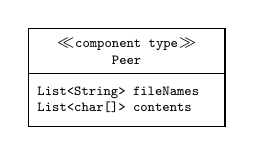
\begin{tikzpicture}[font=\tiny]
	\node[class2] (peer) 
		{\nodepart{one} \stereotype{component type}\\Peer
		 \nodepart{two} 
		 		\tabular{@{}l}
		 			List<String> fileNames\\ 
		 			List<char[]> contents
		 		\endtabular
		 		 };
	\end{tikzpicture}
	\end{column}
\end{columns}

\onslide<10->\textbf{Observation}\\%\vspace{0.1cm}
A component instance can play \textbf{different roles in the same ensemble}.% (at the same time or sequentially).

\end{frame}

\begin{frame}{Components and Roles}
\begin{center}
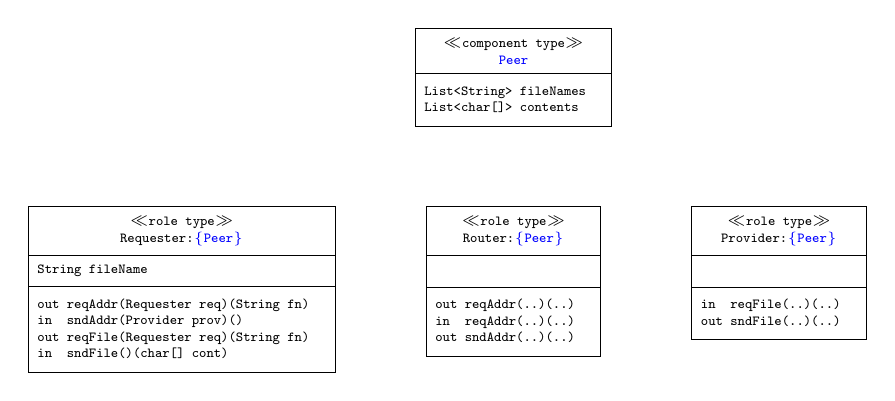
\begin{tikzpicture}[font=\tiny]
	\node[class2] (peer) 
		{\nodepart{one} \stereotype{component type}\\\textcolor{blue}{Peer}
		 \nodepart{two} \tabular{@{}l}
		 		 	List<String> fileNames\\ 
		 		 	List<char[]> contents
		 		 \endtabular
		 		 };
	\node[class3,below left=of peer] (requester)
		{\nodepart{one} \stereotype{role type}\\Requester:\textcolor{blue}{\{Peer\}}
		 \nodepart{two} String fileName
		 \nodepart{three}
		 \tabular{@{}l}
		 	out~reqAddr(Requester req)(String fn)\\
		 	in~~sndAddr(Provider prov)()\\
		 	out~reqFile(Requester req)(String fn)\\
		 	in~~sndFile()(char[] cont)
		 \endtabular
		};
	\node[class3,below=of peer] (router)
		{\nodepart{one} \stereotype{role type}\\Router:\textcolor{blue}{\{Peer\}}
		 \nodepart{two} 
		 \nodepart{three}
		 \tabular{@{}l}
		 	out~reqAddr(..)(..)\\
		 	in~~reqAddr(..)(..)\\
		 	out~sndAddr(..)(..)\\
%		 	in~~sndAddr(..)(..)\\
		 \endtabular
		};
	\node[class3,below right=of peer] (provider)
		{\nodepart{one} \stereotype{role type}\\Provider:\textcolor{blue}{\{Peer\}}
		 \nodepart{two} 
		 \nodepart{three}
		 \tabular{@{}l}
		 	in~~reqFile(..)(..)\\
		 	out~sndFile(..)(..)
		 \endtabular
		};
\end{tikzpicture}
\end{center}

\end{frame}

\begin{frame}{Ensemble Structure without Role Connectors}
\begin{center}
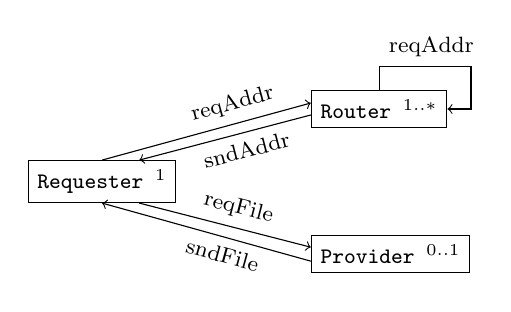
\begin{tikzpicture}[font=\footnotesize]
	\node[ri] (requester) {Requester $^1$};
	\node[ri,above right=of requester,xshift=1cm,yshift=-0.3cm] (router) {Router $^{1..*}$};
	\node[ri,below right=of requester,xshift=1cm,yshift=0.3cm] (provider) {Provider $^{0..1}$};
	
	\draw[->] (requester.north) to node[above,sloped,pos=0.65] {reqAddr} (router.175);
	\draw[<-] (requester.30) to node[below,sloped,pos=0.6] {sndAddr} (router.185);
	
	\draw[->] (requester.330) to node[above,sloped,pos=0.55] {reqFile} (provider.175);
	\draw[<-] (requester.south) to node[below,sloped,pos=0.6] {sndFile} (provider.185);
	
	\draw[->] (router.north) -- node[above right,pos=1] {reqAddr} +(0,0.3) -| ($(router.east) + (0.3,0)$) --  (router.east);
\end{tikzpicture}
\end{center}
\end{frame}


\begin{frame}{Role Behaviors without Role Connectors: Requester}

\begin{center}
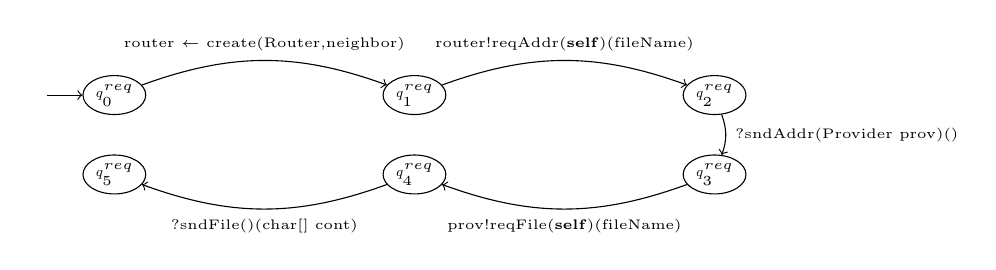
\begin{tikzpicture}
	[font=\tiny,node distance=3cm,]
	\tikzstyle{arrow}=[->,bend left=20];
	\tikzstyle{label}=[auto];
	
	\node (1) [initial,initial text=,state] {$\RoleBehStateVar_0^{req}$};
	\node (2) [state,right=of 1] {$\RoleBehStateVar_1^{req}$};
	\node (3) [state,right=of 2] {$\RoleBehStateVar_2^{req}$};
	\node (4) [state,below=of 3,yshift=2.5cm] {$\RoleBehStateVar_3^{req}$};
	\node (5) [state,left=of 4] {$\RoleBehStateVar_4^{req}$};
	\node (6) [state,left=of 5] {$\RoleBehStateVar_5^{req}$};
	
	\path[arrow,label] 
		(1) edge node {router $\leftarrow$ create(Router,neighbor)} (2)
		(2) edge node {router!reqAddr(\textbf{self})(fileName)} (3)
		(3) edge node {?sndAddr(Provider prov)()} (4)
		(4) edge node {prov!reqFile(\textbf{self})(fileName)} (5)
		(5) edge node {?sndFile()(char[] cont)} (6);
\end{tikzpicture}
\end{center}

%\vspace{2mm}
 $RoleBeh_{Requester} =$\\[0.5em]
\scriptsize{\texttt{router $\leftarrow$ create(Router,neighbor) .\\
	\qquad router!reqAddr(\textbf{self})(fileName) .\\
	\qquad \qquad ?sndAddr(Provider prov)() .\\
	\qquad \qquad \qquad prov!reqFile(\textbf{self})(fileName) .\\
	\qquad \qquad \qquad \qquad ?sndFile()(char[] cont) . \textbf{nil}}}\\
\end{frame}

\begin{frame}{Role Behaviors without Role Connectors: Router and Provider}

 $RoleBeh_{Router} =$\\%[0.5em]
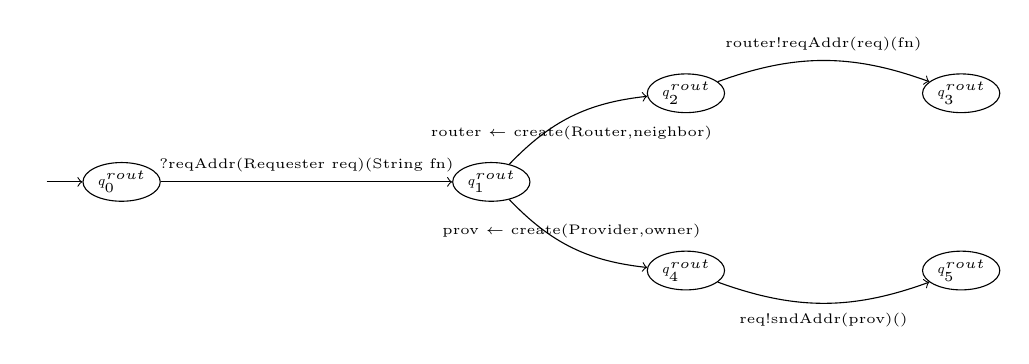
\begin{tikzpicture}[font=\tiny,node distance=2.5cm,]
	
	\tikzstyle{arrow}=[->,bend left=20];
	\tikzstyle{label}=[auto];
	\tikzstyle{arrowbelow}=[->,bend right=20];
	\tikzstyle{labelbelow}=[auto,swap];
	
	\node (1) [initial,initial text=,state] {$\RoleBehStateVar_0^{rout}$};
	\node (2) [state,right=of 1,xshift=1.2cm] {$\RoleBehStateVar_1^{rout}$};
	\node (3) [state,above right=of 2,yshift=-1cm] {$\RoleBehStateVar_2^{rout}$};
	\node (4) [state,right=of 3] {$\RoleBehStateVar_3^{rout}$};
	\node (5) [state,below right=of 2,yshift=1cm] {$\RoleBehStateVar_4^{rout}$};
	\node (6) [state,right=of 5] {$\RoleBehStateVar_5^{rout}$};
	
	\path[->,label]
		(1) edge node {?reqAddr(Requester req)(String fn)} (2);
	\path[arrow,label]
		(2) edge node[below] {router $\leftarrow$ create(Router,neighbor)} (3)
		(3) edge node {router!reqAddr(req)(fn)} (4);
	\path[arrowbelow,labelbelow]
		(2) edge node[above] {prov $\leftarrow$ create(Provider,owner)} (5)
		(5) edge node {req!sndAddr(prov)()} (6);
\end{tikzpicture}

$RoleBeh_{Provider} =$\\
\begin{center}
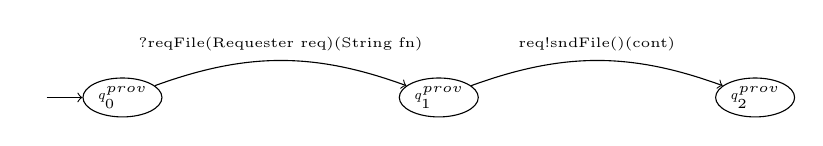
\begin{tikzpicture}
	[font=\tiny,node distance=3cm,]
	\tikzstyle{arrow}=[->,bend left=20];
	\tikzstyle{label}=[auto];
	\node (1) [initial,initial text=,state] {$\RoleBehStateVar_0^{prov}$};
	\node (2) [state,right=of 1] {$\RoleBehStateVar_1^{prov}$};
	\node (3) [state,right=of 2] {$\RoleBehStateVar_2^{prov}$};
	\path[arrow,label] 
		(1) edge node {?reqFile(Requester req)(String fn)} (2)
		(2) edge node {req!sndFile()(cont)} (3);
\end{tikzpicture}
\end{center}
\end{frame}

\begin{frame}{Ensemble Structure with Role Connectors}
\begin{center}
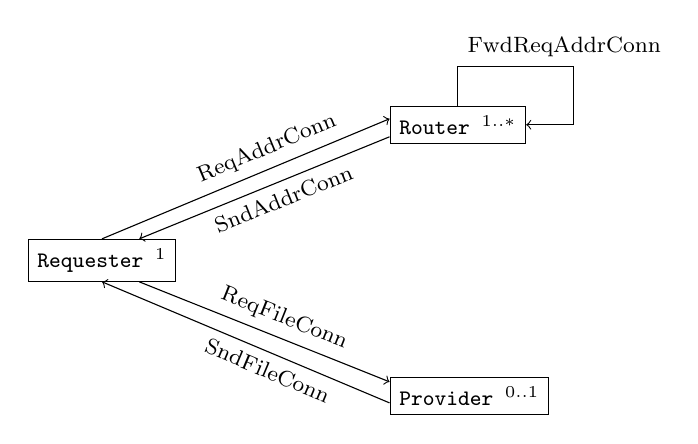
\begin{tikzpicture}[font=\footnotesize]
	\node[ri] (requester) {Requester $^1$};
	\node[ri,above right=of requester,xshift=2cm,yshift=0.5cm] (router) {Router $^{1..*}$};
	\node[ri,below right=of requester,xshift=2cm,yshift=-0.5cm] (provider) {Provider $^{0..1}$};
	
	\draw[->] (requester.north) to node[above,sloped,pos=0.6] {ReqAddrConn} (router.175);
	\draw[<-] (requester.30) to node[below,sloped,pos=0.55] {SndAddrConn} (router.190);
	
	\draw[->] (requester.330) to node[above,sloped,pos=0.55] {ReqFileConn} (provider.170);
	\draw[<-] (requester.south) to node[below,sloped,pos=0.6] {SndFileConn} (provider.185);
	
	\draw[->] (router.north) -- node[above right,pos=1] {FwdReqAddrConn} +(0,0.5) -| ($(router.east) + (0.6,0)$) --  (router.east);
\end{tikzpicture}
\end{center}
\end{frame}


\begin{frame}{Role Behaviors with Role Connectors: Requester}

\begin{center}
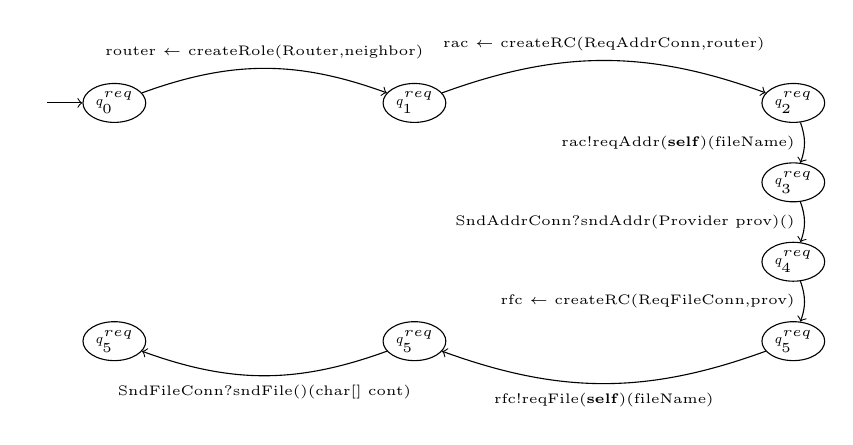
\begin{tikzpicture}
	[font=\tiny,node distance=3cm,]
	\tikzstyle{arrow}=[->,bend left=20];
	\tikzstyle{label}=[auto];
	
	\node (1) [initial,initial text=,state] {$\RoleBehStateVar_0^{req}$};
	\node (2) [state,right=of 1] {$\RoleBehStateVar_1^{req}$};
	\node (3) [state,right=of 2,xshift=1cm] {$\RoleBehStateVar_2^{req}$};
	\node (4) [state,below=of 3,yshift=2.5cm] {$\RoleBehStateVar_3^{req}$};
	\node (5) [state,below=of 4,yshift=2.5cm] {$\RoleBehStateVar_4^{req}$};
	\node (6) [state,below=of 5,yshift=2.5cm] {$\RoleBehStateVar_5^{req}$};
	\node (7) [state,left=of 6, xshift=-1cm] {$\RoleBehStateVar_5^{req}$};
	\node (8) [state,left=of 7] {$\RoleBehStateVar_5^{req}$};
	
	\path[arrow,label] 
		(1) edge node {router $\leftarrow$ createRole(Router,neighbor)} (2)
		(2) edge node {rac $\leftarrow$ createRC(ReqAddrConn,router)} (3)
		(3) edge node[left] {rac!reqAddr(\textbf{self})(fileName)} (4)
		(4) edge node[left] {SndAddrConn?sndAddr(Provider prov)()} (5)
		(5) edge node[left] {rfc $\leftarrow$ createRC(ReqFileConn,prov)} (6)
		(6) edge node {rfc!reqFile(\textbf{self})(fileName)} (7)
		(7) edge node {SndFileConn?sndFile()(char[] cont)} (8);
\end{tikzpicture}
\end{center}

%\vspace{2mm}
 $RoleBeh_{Requester} =$\\[0.5em]
\scriptsize{\texttt{router $\leftarrow$ createRole(Router,neighbor) .\\
	\qquad rac $\leftarrow$ createRC(ReqAddrConn,router) .\\
	\qquad \qquad rac!reqAddr(\textbf{self})(fileName) .\\
	\qquad \qquad \qquad SndAddrConn?sndAddr(Provider prov)() .\\
	\qquad \qquad \qquad \qquad rfc $\leftarrow$ createRC(ReqFileConn,prov) .\\
	\qquad \qquad \qquad \qquad \qquad rfc!reqFile(\textbf{self})(fileName) .\\
	\qquad \qquad \qquad \qquad \qquad \qquad SndFileConn?sndFile()(char[] cont) . \textbf{nil}}}\\
\end{frame}

\begin{frame}{Role Behaviors with Role Connectors: Router}

 $RoleBeh_{Router} =$\\%[0.5em]
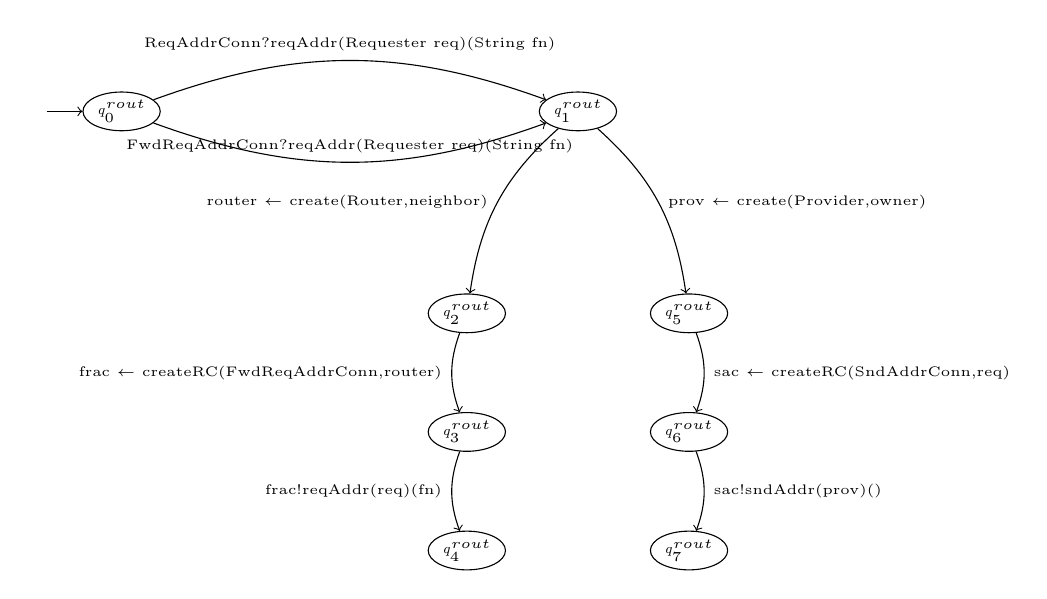
\begin{tikzpicture}[font=\tiny,node distance=1cm,]
	
	\tikzstyle{arrow}=[->,bend right=20];
	\tikzstyle{label}=[auto];
	\tikzstyle{arrowbelow}=[->,bend left=20];
	\tikzstyle{labelbelow}=[auto];
	
	\node (1) [initial,initial text=,state] {$\RoleBehStateVar_0^{rout}$};
	\node (2) [state,right=of 1,xshift=3.8cm] {$\RoleBehStateVar_1^{rout}$};
	\node (3) [state,below left=of 2,yshift=-1.5cm] {$\RoleBehStateVar_2^{rout}$};
	\node (4) [state,below=of 3] {$\RoleBehStateVar_3^{rout}$};
	\node (5) [state,below=of 4] {$\RoleBehStateVar_4^{rout}$};
	\node (6) [state,below right=of 2,yshift=-1.5cm] {$\RoleBehStateVar_5^{rout}$};
	\node (7) [state,below=of 6] {$\RoleBehStateVar_6^{rout}$};
	\node (8) [state,below=of 7] {$\RoleBehStateVar_7^{rout}$};
	
	
	\path[arrowbelow,labelbelow]
		(1) edge node[above] {ReqAddrConn?reqAddr(Requester req)(String fn)} (2);
	\path[arrow,label]
		(1) edge node {FwdReqAddrConn?reqAddr(Requester req)(String fn)} (2);
	\path[arrow,label,left]
		(2) edge node {router $\leftarrow$ create(Router,neighbor)} (3)
		(3) edge node {frac $\leftarrow$ createRC(FwdReqAddrConn,router)} (4)
		(4) edge node {frac!reqAddr(req)(fn)} (5);
	\path[arrowbelow,labelbelow,right]
		(2) edge node {prov $\leftarrow$ create(Provider,owner)} (6)
		(6) edge node {sac $\leftarrow$ createRC(SndAddrConn,req)} (7)
		(7) edge node {sac!sndAddr(prov)()} (8);
\end{tikzpicture}
\end{frame}

\begin{frame}{Role Behaviors with Role Connectors: Provider}
$RoleBeh_{Provider} =$\\
\begin{center}
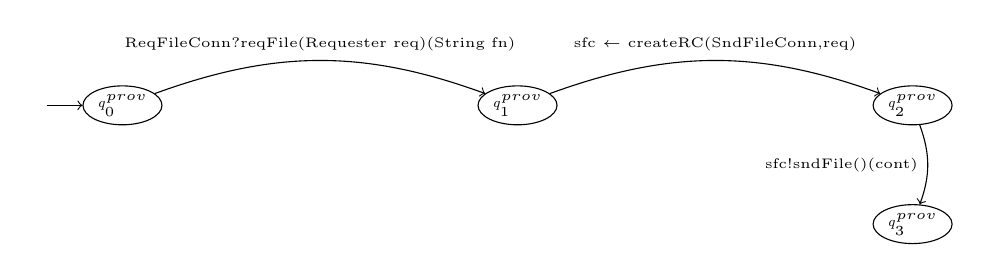
\begin{tikzpicture}
	[font=\tiny,node distance=4cm,]
	\tikzstyle{arrow}=[->,bend left=20];
	\tikzstyle{label}=[auto];
	\node (1) [initial,initial text=,state] {$\RoleBehStateVar_0^{prov}$};
	\node (2) [state,right=of 1] {$\RoleBehStateVar_1^{prov}$};
	\node (3) [state,right=of 2] {$\RoleBehStateVar_2^{prov}$};
	\node (4) [state,below=of 3,yshift=3cm] {$\RoleBehStateVar_3^{prov}$};
	\path[arrow,label] 
		(1) edge node {ReqFileConn?reqFile(Requester req)(String fn)} (2)
		(2) edge node {sfc $\leftarrow$ createRC(SndFileConn,req)} (3)
		(3) edge node[left] {sfc!sndFile()(cont)} (4);
\end{tikzpicture}
\end{center}
\end{frame}

\end{document}

%%% Local Variables: 
%%% mode: latex
%%% TeX-PDF-mode: t
%%% End: 